%% ═══════════════════════════════════════════════════════════════════════════
%% PBEOT504: DATABASE MANAGEMENT SYSTEM — MODULE 1 COMPREHENSIVE STUDY NOTES
%% APJ Abdul Kalam Technological University / CET S5 (2024 Scheme)
%% Styled with Anthropic Notes Design System
%% ═══════════════════════════════════════════════════════════════════════════

\documentclass[11pt,a4paper]{article}

%% ─── Packages ────────────────────────────────────────────────────────────────
\usepackage{fontspec}

%% Font configuration with local fonts and synthetic fallbacks
\setmainfont{Anthropic-serif}[
    Path          = ./,
    Extension     = .ttf,
    AutoFakeBold  = 1.5,
    AutoFakeSlant = 0.2
]
\setsansfont{Poppins}[
    AutoFakeBold  = 1.5,
    AutoFakeSlant = 0.2
]
\setmonofont{DejaVu Sans Mono}[Scale=MatchLowercase]

\usepackage[margin=2.0cm, top=2.5cm, bottom=2.5cm, headheight=25pt]{geometry}
\usepackage[table]{xcolor}
\usepackage{tikz}
\usetikzlibrary{shapes.geometric, arrows.meta, positioning, fit, backgrounds,
                decorations.pathreplacing, calc, patterns}
\usepackage{listings}
\usepackage{tcolorbox}
\tcbuselibrary{listings, skins, breakable, raster}
\usepackage{fancyhdr}
\usepackage{titlesec}
\usepackage{titletoc}
\usepackage{enumitem}
\usepackage{booktabs}
\usepackage{tabularx}
\usepackage{array}
\usepackage{microtype}
\usepackage{hyperref}
\usepackage{amssymb}
\usepackage{amsmath}
\usepackage{parskip}
\usepackage{colortbl}
\usepackage[normalem]{ulem}

%% ─── Document Metadata ──────────────────────────────────────────────────────
\newcommand{\docsubject}{PBEOT504: Database Management System (S5)}
\newcommand{\docshortsubject}{PBEOT504 · Mod 1}
\newcommand{\doctitle}{Database Concepts, ER Modeling \& Physical Storage}
\newcommand{\docauthor}{Sudheesh}

%% ─── Widow / Orphan Protection ──────────────────────────────────────────────
\widowpenalty=10000
\clubpenalty=10000

%% ─── Spacing ────────────────────────────────────────────────────────────────
\setlength{\parskip}{0.45em plus 0.15em minus 0.1em}
\setlength{\parindent}{0pt}

%% ─── Table Geometry ─────────────────────────────────────────────────────────
\setlength{\aboverulesep}{0pt}
\setlength{\belowrulesep}{0pt}
\setlength{\extrarowheight}{0.65ex}
\renewcommand{\arraystretch}{1.4}
\setlength{\arrayrulewidth}{0.4pt}

\newcolumntype{L}[1]{>{\raggedright\arraybackslash}p{#1}}
\newcolumntype{C}[1]{>{\centering\arraybackslash}p{#1}}
\newcolumntype{R}[1]{>{\raggedleft\arraybackslash}p{#1}}

%% ─── Brand Colors (Anthropic Palette) ────────────────────────────────────────
\definecolor{AnthDark}{HTML}{141413}
\definecolor{AnthLight}{HTML}{faf9f5}
\definecolor{AnthMidGray}{HTML}{7a7870}
\definecolor{AnthLightGray}{HTML}{e8e6dc}
\definecolor{AnthOrange}{HTML}{d97757}
\definecolor{AnthBlue}{HTML}{3b75a4}
\definecolor{AnthGreen}{HTML}{5d7343}
\definecolor{AnthCodeBG}{HTML}{edebe1}
\definecolor{AnthCardBG}{HTML}{f6f5ee}

\arrayrulecolor{AnthMidGray!40}

%% ─── Hyperref ────────────────────────────────────────────────────────────────
\hypersetup{
  colorlinks  = true,
  linkcolor   = AnthBlue,
  urlcolor    = AnthOrange,
  citecolor   = AnthGreen,
  pdftitle    = {\doctitle{} · \docsubject},
  pdfauthor   = {\docauthor},
}

%% ─── Page Style ─────────────────────────────────────────────────────────────
\pagestyle{fancy}
\fancyhf{}
\fancyhead[L]{\small\sffamily\color{AnthMidGray}\textbf{\doctitle} \textbar\ \docshortsubject}
\fancyhead[R]{\small\sffamily\color{AnthMidGray}\thepage}
\renewcommand{\headrulewidth}{0.4pt}
\renewcommand{\headrule}{%
  \hbox to\headwidth{\color{AnthOrange}\leaders\hrule height \headrulewidth\hfill}}
\renewcommand{\footrulewidth}{0.4pt}
\renewcommand{\footrule}{%
  \hbox to\headwidth{\color{AnthLightGray}\leaders\hrule height \footrulewidth\hfill}}
\fancyfoot[L]{\footnotesize\sffamily\color{AnthMidGray} APJ Abdul Kalam Technological University (KTU S5)}
\fancyfoot[R]{\footnotesize\sffamily\color{AnthMidGray} PBEOT504 Study Material}

%% ─── Section Formatting ─────────────────────────────────────────────────────
\titleformat{\section}
  {\Large\bfseries\sffamily\color{AnthDark}}
  {\colorbox{AnthOrange}{\makebox[0.65cm][c]{\color{white}\thesection}}\quad}
  {0em}
  {}
  [\vspace{-0.5ex}\color{AnthLightGray}\hrule\vspace{0.4ex}]

\titleformat{\subsection}
  {\large\bfseries\sffamily\color{AnthDark}}
  {\color{AnthBlue}\thesubsection\enspace}
  {0em}{}

\titleformat{\subsubsection}
  {\normalsize\bfseries\sffamily\color{AnthDark}}
  {\color{AnthGreen}\thesubsubsection\enspace}
  {0em}{}

\titlespacing{\section}     {0pt}{1.5em}{0.6em}
\titlespacing{\subsection}  {0pt}{1.1em}{0.3em}
\titlespacing{\subsubsection}{0pt}{0.8em}{0.25em}

%% ─── Table of Contents Styling ──────────────────────────────────────────────
\contentsmargin{0pt}

\titlecontents{section}
  [0pt]
  {\vspace{4pt}\bfseries\sffamily\color{AnthDark}}
  {\colorbox{AnthOrange}{\makebox[0.55cm][c]{\color{white}\small\thecontentslabel}}\enspace}
  {}
  {\hfill\color{AnthOrange}\contentspage}

\titlecontents{subsection}
  [1.5em]
  {\small\sffamily\color{AnthBlue}}
  {\thecontentslabel\enspace}
  {}
  {\titlerule*[6pt]{\tiny\color{AnthMidGray}.}\color{AnthBlue}\contentspage}

\titlecontents{subsubsection}
  [3.5em]
  {\footnotesize\sffamily\color{AnthGreen}}
  {\thecontentslabel\enspace}
  {}
  {\titlerule*[6pt]{\tiny\color{AnthMidGray}.}\color{AnthGreen}\contentspage}

%% ─── tcolorbox Styles ───────────────────────────────────────────────────────
\tcbset{
  notebox/.style={
    enhanced, breakable,
    colback     = AnthCardBG,
    colframe    = AnthMidGray,
    arc=4pt, outer arc=4pt,
    sharp corners=west,
    left=9pt, right=9pt, top=7pt, bottom=7pt,
    boxrule     = 0.5pt,
    colupper    = AnthDark,
    fonttitle   = \bfseries\sffamily\small,
    coltitle    = AnthDark,
    colbacktitle= AnthLightGray,
    borderline west={3pt}{0pt}{AnthMidGray},
    drop fuzzy shadow={AnthMidGray!20},
  },
  tipbox/.style={
    enhanced, breakable,
    colback     = AnthGreen!8,
    colframe    = AnthGreen!70,
    arc=4pt, outer arc=4pt,
    sharp corners=west,
    left=9pt, right=9pt, top=7pt, bottom=7pt,
    boxrule     = 0.5pt,
    colupper    = AnthDark,
    fonttitle   = \bfseries\sffamily\small,
    coltitle    = white,
    colbacktitle= AnthGreen,
    borderline west={3pt}{0pt}{AnthGreen},
    drop fuzzy shadow={AnthGreen!20},
  },
  warnbox/.style={
    enhanced, breakable,
    colback     = AnthOrange!7,
    colframe    = AnthOrange!70,
    arc=4pt, outer arc=4pt,
    sharp corners=west,
    left=9pt, right=9pt, top=7pt, bottom=7pt,
    boxrule     = 0.5pt,
    colupper    = AnthDark,
    fonttitle   = \bfseries\sffamily\small,
    coltitle    = white,
    colbacktitle= AnthOrange,
    borderline west={3pt}{0pt}{AnthOrange},
    drop fuzzy shadow={AnthOrange!20},
  },
  defbox/.style={
    enhanced, breakable,
    colback     = AnthLight,
    colframe    = AnthLightGray,
    arc=4pt, outer arc=4pt,
    sharp corners=west,
    left=9pt, right=9pt, top=7pt, bottom=7pt,
    boxrule     = 0.5pt,
    colupper    = AnthDark,
    borderline west={3.5pt}{0pt}{AnthOrange},
    drop fuzzy shadow={AnthMidGray!20},
  },
  derivbox/.style={
    enhanced, breakable,
    colback     = AnthCardBG!60,
    colframe    = AnthBlue!70,
    arc=4pt, outer arc=4pt,
    sharp corners=west,
    left=9pt, right=9pt, top=7pt, bottom=7pt,
    boxrule     = 0.5pt,
    colupper    = AnthDark,
    fonttitle   = \bfseries\sffamily\small,
    coltitle    = white,
    colbacktitle= AnthBlue,
    borderline west={3.5pt}{0pt}{AnthBlue},
    drop fuzzy shadow={AnthBlue!15},
  },
  problembox/.style={
    enhanced, breakable,
    colback     = AnthBlue!6,
    colframe    = AnthBlue!80,
    arc=4pt, outer arc=4pt,
    sharp corners=west,
    left=9pt, right=9pt, top=7pt, bottom=7pt,
    boxrule     = 0.5pt,
    colupper    = AnthDark,
    fonttitle   = \bfseries\sffamily\small,
    coltitle    = white,
    colbacktitle= AnthBlue,
    borderline west={3.5pt}{0pt}{AnthBlue},
    drop fuzzy shadow={AnthBlue!20},
  },
  solbox/.style={
    enhanced, breakable,
    colback     = AnthLight,
    colframe    = AnthGreen!60,
    arc=4pt, outer arc=4pt,
    sharp corners=west,
    left=9pt, right=9pt, top=7pt, bottom=7pt,
    boxrule     = 0.5pt,
    colupper    = AnthDark,
    fonttitle   = \bfseries\sffamily\small,
    coltitle    = white,
    colbacktitle= AnthGreen!85,
    borderline west={3.5pt}{0pt}{AnthGreen},
    drop fuzzy shadow={AnthGreen!15},
  }
}

%% ─── Inline Helpers & Custom Environments ────────────────────────────────────
\newcommand{\ic}[1]{\mbox{\colorbox{AnthCodeBG}{\footnotesize\ttfamily\textcolor{AnthBlue}{#1}}}}

\newcommand{\concept}[1]{%
  \vspace{3pt}\noindent\textcolor{AnthGreen}{\rule{3.5pt}{10pt}}\enspace
  \textbf{\sffamily\color{AnthDark}#1}\par\vspace{2pt}%
}

\newcommand{\syllabusitem}[1]{%
  \begin{tcolorbox}[enhanced, colback=AnthOrange!8, colframe=AnthOrange, boxrule=0.4pt, arc=3pt, left=7pt, right=7pt, top=3pt, bottom=3pt]
    \small\sffamily\textbf{\color{AnthOrange}Syllabus Requirement:} #1
  \end{tcolorbox}
}

\newenvironment{Note}[1][Note]{\begin{tcolorbox}[notebox, title=#1]}{\end{tcolorbox}}
\newenvironment{Tip}[1][Key Concept / Design Rule]{\begin{tcolorbox}[tipbox, title=#1]}{\end{tcolorbox}}
\newenvironment{Warn}[1][Important Exam Alert]{\begin{tcolorbox}[warnbox, title=#1]}{\end{tcolorbox}}
\newenvironment{Def}[1][]{\begin{tcolorbox}[defbox]\ifx&#1&\else\textbf{\color{AnthOrange}#1:}\enspace\fi}{\end{tcolorbox}}
\newenvironment{Deriv}[1][Analysis \& Comparison]{\begin{tcolorbox}[derivbox, title=#1]}{\end{tcolorbox}}
\newenvironment{Problem}[1][Problem Scenario]{\begin{tcolorbox}[problembox, title=#1]}{\end{tcolorbox}}
\newenvironment{Solution}[1][Step-by-Step Solution]{\begin{tcolorbox}[solbox, title=#1]}{\end{tcolorbox}}

%% ─── Lists Styling ──────────────────────────────────────────────────────────
\setlist[itemize,1]{itemsep=1.5pt, topsep=2pt, parsep=0pt, label={\color{AnthOrange}\small$\blacktriangleright$}}
\setlist[itemize,2]{itemsep=1.5pt, topsep=2pt, parsep=0pt, label={\color{AnthBlue}\small$\blacktriangleright$}}
\setlist[itemize,3]{itemsep=1.5pt, topsep=2pt, parsep=0pt, label={\color{AnthGreen}\small$\blacktriangleright$}}

\setlist[enumerate,1]{itemsep=1.5pt, topsep=2pt, parsep=0pt, label={\bfseries\color{AnthOrange}\arabic*.}}
\setlist[enumerate,2]{itemsep=1.5pt, topsep=2pt, parsep=0pt, label={\bfseries\color{AnthBlue}(\alph*)}}
\setlist[enumerate,3]{itemsep=1.5pt, topsep=2pt, parsep=0pt, label={\color{AnthGreen}\roman*.}}

%% ─── Title Page Macro ───────────────────────────────────────────────────────
\newcommand{\maketitlepage}{%
  \begin{titlepage}
    \pagecolor{AnthDark}
    \color{AnthLight}
    \vspace*{2.2cm}
    \begin{center}
      {\huge\bfseries\sffamily \doctitle}\\[0.8em]
      {\Large\sffamily\color{AnthOrange} \docsubject}\\[0.4em]
      {\large\sffamily\color{AnthMidGray} Bachelor of Technology (B.Tech) — 2024 Scheme}\\[2.0em]
      \color{AnthOrange}\rule{0.5\textwidth}{1.2pt}\\[1.8em]
      {\normalsize\sffamily\color{AnthLightGray} Complete Technical Notes, Schema Architectures \& ER Design Suite}\\[0.4em]
      {\small\sffamily\color{AnthMidGray} Prepared from Course Materials, Lecture Slides \& KTU Curriculum}\\[2.8em]
      \begin{tcolorbox}[enhanced, width=0.84\textwidth, colback=AnthDark!90, colframe=AnthOrange!60, arc=4pt, boxrule=0.6pt]
        \centering\small\sffamily\color{AnthLight}
        \textbf{Module 1 Complete Syllabus Coverage:}\\[3pt]
        $\bullet$ Concepts \& Overview of DBMS: File Processing vs DBMS, Data Independence\\
        $\bullet$ Structured, Semi-Structured \& Unstructured Data, Three-Schema Architecture\\
        $\bullet$ Database Languages (DDL, DML, DCL, VDL), Interfaces \& DBMS Classifications\\
        $\bullet$ Entity-Relationship (ER) Model: Entities, Attributes, Relationships, Constraints\\
        $\bullet$ Weak Entities, Identifying Relationships, $(min, max)$ \& Ternary Relationships\\
        $\bullet$ Physical Data Organization: Blocking Factors, Heap Files \& Indexing Calculations
      \end{tcolorbox}
      \vfill
      {\small\sffamily\color{AnthMidGray} Compiled \today}
    \end{center}
    \vspace*{0.8cm}
  \end{titlepage}
  \pagecolor{AnthLight}
  \color{AnthDark}
}

%% ═══════════════════════════════════════════════════════════════════════════
%% DOCUMENT BODY
%% ═══════════════════════════════════════════════════════════════════════════
\begin{document}

\maketitlepage

%% ─── Table of Contents ───────────────────────────────────────────────────────
\thispagestyle{empty}
{
  \hypersetup{hidelinks}
  \tableofcontents
}
\clearpage

%% ─────────────────────────────────────────────────────────────────────────────
\section{Database System Concepts and Architecture}
%% ─────────────────────────────────────────────────────────────────────────────

\syllabusitem{Concept \& Overview of Database Management Systems (DBMS) - Characteristics of Database system, Structured, semi-structured and unstructured data. Data Models and Schema - Three Schema architecture. Database Languages.}

\subsection{Introduction: File Processing Systems vs. Database Approach}

Before the advent of Database Management Systems (DBMS), organizations stored data in traditional operating system flat files. In a \textbf{File-Processing System}, each application department maintained its own private data files along with custom programs to process them.

\concept{Limitations of Traditional File Processing}
\begin{enumerate}
  \item \textbf{Data Redundancy and Inconsistency:} The same data (e.g., student address) is duplicated across multiple department files. Updating one file without updating others leads to conflicting, inconsistent records.
  \item \textbf{Program-Data Dependence:} The structure of data records is hardcoded directly into application programs. Modifying a record format requires rewriting and recompiling all dependent application programs.
  \item \textbf{Difficulty in Accessing Data:} Ad-hoc queries (e.g., finding all students with GPA $> 3.5$ from a specific district) require writing entirely new application programs from scratch.
  \item \textbf{Data Isolation and Lack of Standards:} Data is scattered in various file formats (binary, text, delimited), making data integration and cross-department queries exceptionally difficult.
  \item \textbf{Integrity and Validation Problems:} Business rules (e.g., account balance $\ge 0$) must be hardcoded inside every application program rather than enforced uniformly at the data level.
  \item \textbf{Atomicity and Recovery Issues:} A system crash in the middle of a fund transfer may leave funds deducted from Account A without being credited to Account B.
  \item \textbf{Concurrent Access Anomalies:} Uncontrolled simultaneous updates by multiple users lead to lost updates, dirty reads, and corrupted files.
  \item \textbf{Security Problems:} Difficult to enforce granular user-level authorization and access control on raw operating system files.
\end{enumerate}

\begin{Def}[Database and DBMS Defined]
A \textbf{Database} is an organized, logically coherent collection of related data with some inherent meaning, designed to represent a mini-world (Universe of Discourse - UoD).\\
A \textbf{Database Management System (DBMS)} is a collection of generalized software programs that facilitates the processes of defining, constructing, manipulating, and sharing databases among various users and applications.
\end{Def}

%% ─────────────────────────────────────────────────────────────────────────────
\subsection{Characteristics of the Database Approach}

The database approach possesses four fundamental characteristics that differentiate it from traditional file processing:

\begin{center}
\resizebox{0.92\textwidth}{!}{%
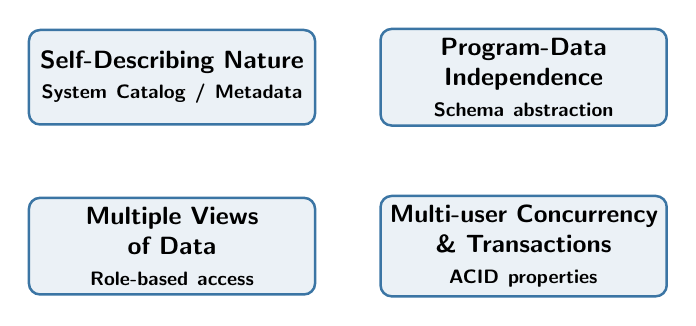
\begin{tikzpicture}[
  node distance=0.7cm and 0.8cm,
  block/.style={rectangle, draw=AnthDark, fill=AnthCardBG, rounded corners=3pt, line width=0.6pt, text width=3.2cm, align=center, minimum height=1.1cm, font=\small\sffamily},
  majorblock/.style={rectangle, draw=AnthBlue, fill=AnthBlue!10, rounded corners=4pt, line width=0.9pt, text width=3.4cm, align=center, minimum height=1.2cm, font=\small\sffamily\bfseries}
]
  \node[majorblock] (c1) {Self-Describing Nature\\ \scriptsize\sffamily System Catalog / Metadata};
  \node[majorblock, right=of c1] (c2) {Program-Data\\ Independence\\ \scriptsize\sffamily Schema abstraction};
  \node[majorblock, below=0.9cm of c1] (c3) {Multiple Views\\ of Data\\ \scriptsize\sffamily Role-based access};
  \node[majorblock, right=of c3] (c4) {Multi-user Concurrency\\ \& Transactions\\ \scriptsize\sffamily ACID properties};
\end{tikzpicture}%
}
\end{center}

\begin{enumerate}
  \item \textbf{Self-Describing Nature of a Database System:}
    A DBMS stores not only the operational data itself, but also a complete definition of the database structure, data types, constraints, and relationships. This descriptive data is called \textbf{Metadata} and is maintained in the \textbf{System Catalog (Data Dictionary)}.
  \item \textbf{Insulation Between Programs and Data (Program-Data Independence):}
    The internal storage format and access paths can be modified without altering user application programs. The DBMS provides abstract interfaces so that programs refer to conceptual entities rather than physical byte offsets.
  \item \textbf{Support for Multiple User Views:}
    A database has many distinct user groups (e.g., Students, Faculty, Accounts, Registrar). Each group requires a specialized, tailored perspective of the database. A view may present a virtual table derived from base tables while filtering out confidential fields.
  \item \textbf{Sharing of Data and Multi-User Transaction Processing:}
    A multi-user DBMS enforces concurrency control mechanisms (locking, timestamps) ensuring that concurrent operations execute safely without interference, guaranteeing the \textbf{ACID Properties (Atomicity, Consistency, Isolation, Durability)}.
\end{enumerate}

%% ─────────────────────────────────────────────────────────────────────────────
\subsection{Classification of Data: Structured, Semi-Structured, and Unstructured}

\begin{center}
\small
\begin{tabularx}{\textwidth}{L{2.5cm} L{3.8cm} L{3.5cm} X}
  \rowcolor{AnthDark}
  \color{white}\textbf{Data Category} & \color{white}\textbf{Structural Organization} & \color{white}\textbf{Data Formats} & \color{white}\textbf{DBMS Technology} \\
  \rowcolor{AnthCardBG} \textbf{Structured Data} & Strict pre-defined schema with rigid tables, rows, and strongly typed columns & Relational tables, SQL records, Fixed-width CSV & Relational DBMS (Oracle, PostgreSQL, MySQL) \\
  \textbf{Semi-Structured Data} & Self-describing schema embedded within data; tags and key-value hierarchies & JSON, XML, BSON, YAML & Document \& Key-Value NoSQL (MongoDB, Redis, CouchDB) \\
  \rowcolor{AnthCardBG} \textbf{Unstructured Data} & No pre-defined conceptual schema or tabular model; heavy raw content & Plain text, PDF, images, video, audio streams, sensor logs & Object Storage, Vector DBs, Graph DBs, Data Lakes \\
\end{tabularx}
\end{center}

%% ─────────────────────────────────────────────────────────────────────────────
\subsection{Data Models, Schemas, and Instances}

\concept{Data Model Categories}
A data model is a collection of concepts used to describe the structure of a database (data types, relationships, constraints, and basic operations).
\begin{enumerate}
  \item \textbf{Conceptual / High-Level Data Models:} Provide concepts close to how users perceive data (e.g., Entity-Relationship Model, Object Model).
  \item \textbf{Representational / Implementation Data Models:} Concepts easily understood by end-users that map directly to physical computer storage (e.g., Relational Model, Network Model, Hierarchical Model).
  \item \textbf{Physical / Low-Level Data Models:} Describe how data is stored on disk drives as records, blocks, orderings, and access paths (indexes).
\end{enumerate}

\concept{Database Schema vs. Database State (Instance)}
\begin{itemize}
  \item \textbf{Database Schema (Intension):} The overall structural description of the database specified during design phase. It rarely changes. E.g., $\text{STUDENT}(\underline{\text{RollNo}}, \text{Name}, \text{Age}, \text{Branch})$.
  \item \textbf{Database State / Instance (Extension):} The actual data stored in the database at a specific snapshot in time. It changes constantly as records are inserted, deleted, or updated.
\end{itemize}

%% ─────────────────────────────────────────────────────────────────────────────
\subsection{The Three-Schema Architecture and Data Independence}

The ANSI/SPARC \textbf{Three-Schema Architecture} separates user application interfaces from the physical database to achieve program-data independence.

\begin{center}
\resizebox{0.7\textwidth}{!}{%
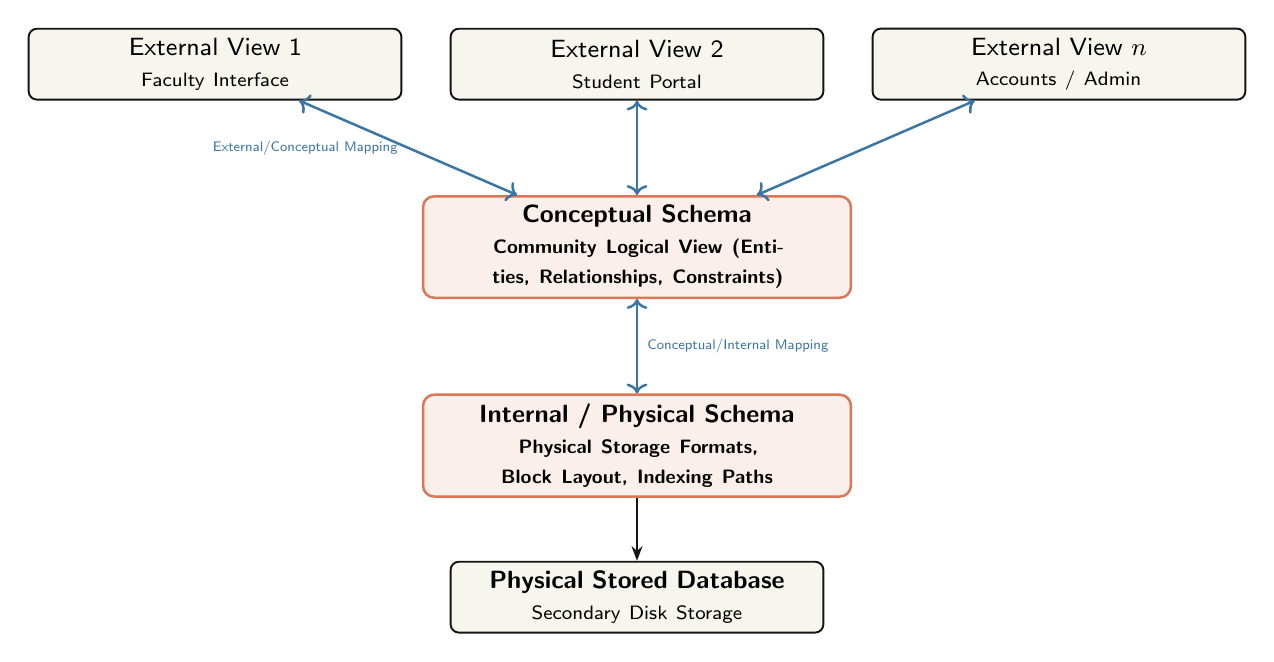
\begin{tikzpicture}[
  block/.style={rectangle, draw=AnthDark, fill=AnthCardBG, rounded corners=3pt, line width=0.7pt, text width=4.5cm, align=center, minimum height=0.9cm, font=\small\sffamily},
  majorblock/.style={rectangle, draw=AnthOrange, fill=AnthOrange!12, rounded corners=4pt, line width=0.9pt, text width=5.2cm, align=center, minimum height=1.0cm, font=\small\sffamily\bfseries},
  arrow/.style={<->, line width=0.9pt, color=AnthBlue}
]
  \node[block] (ext1) {External View 1\\ \scriptsize Faculty Interface};
  \node[block, right=0.6cm of ext1] (ext2) {External View 2\\ \scriptsize Student Portal};
  \node[block, right=0.6cm of ext2] (ext3) {External View $n$\\ \scriptsize Accounts / Admin};

  \node[majorblock, below=1.2cm of ext2] (conc) {\textbf{Conceptual Schema}\\ \scriptsize Community Logical View (Entities, Relationships, Constraints)};
  \node[majorblock, below=1.2cm of conc] (internal) {\textbf{Internal / Physical Schema}\\ \scriptsize Physical Storage Formats, Block Layout, Indexing Paths};
  \node[block, below=0.8cm of internal] (db) {\textbf{Physical Stored Database}\\ \scriptsize Secondary Disk Storage};

  \draw[arrow] (ext1) -- node[left, font=\tiny\sffamily]{External/Conceptual Mapping} (conc);
  \draw[arrow] (ext2) -- (conc);
  \draw[arrow] (ext3) -- (conc);
  \draw[arrow] (conc) -- node[right, font=\tiny\sffamily]{Conceptual/Internal Mapping} (internal);
  \draw[line width=0.8pt, -{Stealth[scale=0.8]}, color=AnthDark] (internal) -- (db);
\end{tikzpicture}%
}
\end{center}

\concept{The Three Schema Levels}
\begin{enumerate}
  \item \textbf{External Level (User Views):} Describes the part of the database relevant to a specific user group while concealing the rest of the database.
  \item \textbf{Conceptual Level (Community Logical View):} Describes the structure of the entire database for a community of users, defining entities, data types, relationships, user operations, and semantic constraints without referencing physical storage details.
  \item \textbf{Internal Level (Physical Storage Schema):} Describes the complete physical storage structure, record formats, page allocations, clustering, and access paths (indexes).
\end{enumerate}

\concept{Data Independence}
Data independence is the capacity to change the schema at one level of a database system without having to alter the schema at the next higher level.

\begin{Def}[Logical vs. Physical Data Independence]
\textbf{1. Logical Data Independence:}
The capacity to modify the \textbf{conceptual schema} without having to change external schemas or rewrite existing application programs.\\
\emph{Examples:} Adding a new entity type or attribute, deleting an unused attribute, expanding relationship constraints.\\
\emph{Note:} Challenging to achieve because application programs are heavily coupled to logical structures.\\

\textbf{2. Physical Data Independence:}
The capacity to modify the \textbf{internal schema} without having to change the conceptual or external schemas.\\
\emph{Examples:} Creating a new B+ tree index, changing physical file organization from heap to hashed, reorganizing disk blocks, switching storage hardware.\\
\emph{Note:} Easy to achieve; only internal-to-conceptual mapping rules need adjustment.
\end{Def}

%% ─────────────────────────────────────────────────────────────────────────────
\subsection{Database Languages and User Classifications}

\concept{Database Languages}
\begin{itemize}
  \item \textbf{DDL (Data Definition Language):} Used by DBAs and designers to define conceptual and internal schemas (e.g., \ic{CREATE}, \ic{ALTER}, \ic{DROP}).
  \item \textbf{DML (Data Manipulation Language):} Used to retrieve, insert, delete, and modify data:
    \begin{itemize}
      \item \emph{High-Level / Non-procedural (Declarative) DML:} Specifies \textbf{what} data to retrieve rather than \textbf{how} to retrieve it (e.g., SQL). Processes sets of records simultaneously.
      \item \emph{Low-Level / Procedural DML:} Embedded in general-purpose programming languages; retrieves individual records one at a time and specifies exact navigation procedures.
    \end{itemize}
  \item \textbf{VDL (View Definition Language):} Specifies user views and their mappings to the conceptual schema.
  \item \textbf{DCL (Data Control Language):} Controls user privileges and transaction states (e.g., \ic{GRANT}, \ic{REVOKE}, \ic{COMMIT}, \ic{ROLLBACK}).
\end{itemize}

\concept{Database Users}
\begin{enumerate}
  \item \textbf{Database Administrator (DBA):} Responsible for authorizing database access, monitoring performance, acquiring hardware/software resources, managing security, and overseeing backup/recovery.
  \item \textbf{Database Designers:} Identify data requirements, choose appropriate data models, and create conceptual and physical schemas.
  \item \textbf{End Users:} People whose jobs require access to the database (Casual users, Naive/Parametric users accessing predefined canned transactions, Sophisticated analysts).
  \item \textbf{Application Programmers:} Software engineers who write DML queries embedded in host programming languages (Java, Python, C++) to build business applications.
\end{enumerate}

%% ─────────────────────────────────────────────────────────────────────────────
\clearpage
\section{The Entity-Relationship (ER) Conceptual Model}
%% ─────────────────────────────────────────────────────────────────────────────

\syllabusitem{ER model - Basic concepts, entity set \& attributes, notations, Relationships and constraints, cardinality, participation, notations, weak entities, relationships of degree 3.}

\subsection{Basic Concepts: Entities, Attributes, and Keys}

The \textbf{Entity-Relationship (ER) Model} is a high-level conceptual data model introduced by Peter Chen in 1976. It represents the enterprise schema graphically as entities, attributes, and relationships.

\concept{1. Entities and Entity Sets}
\begin{itemize}
  \item \textbf{Entity:} A distinct "thing" or "object" in the real world that is distinguishable from other objects (e.g., a particular employee \emph{John Smith}, a specific department \emph{Research}).
  \item \textbf{Entity Type:} A collection of entities that share the same attributes (e.g., \ic{EMPLOYEE}, \ic{DEPARTMENT}).
  \item \textbf{Entity Set:} The current collection of all entities of a particular entity type stored in the database at any moment.
\end{itemize}

\concept{2. Types of Attributes}
\begin{center}
\small
\begin{tabularx}{\textwidth}{L{3.0cm} L{3.5cm} X L{3.0cm}}
  \rowcolor{AnthDark}
  \color{white}\textbf{Attribute Type} & \color{white}\textbf{Definition} & \color{white}\textbf{Real-World Example} & \color{white}\textbf{ER Diagram Notation} \\
  \rowcolor{AnthCardBG} \textbf{Simple (Atomic)} & Cannot be divided into smaller components & \ic{Age}, \ic{Salary}, \ic{Gender} & Single Oval \\
  \textbf{Composite} & Can be divided into smaller sub-components & \ic{Name} $\to$ (\ic{First\_Name}, \ic{Last\_Name}); \ic{Address} $\to$ (\ic{Street}, \ic{City}) & Tree of connected Ovals \\
  \rowcolor{AnthCardBG} \textbf{Single-Valued} & Has exactly one single value for an entity & \ic{SSN}, \ic{DOB}, \ic{RollNo} & Single Oval \\
  \textbf{Multi-Valued} & Can have a set of multiple values for an entity & \ic{Phone\_Numbers}, \ic{College\_Degrees} & \textbf{Double Oval} \\
  \rowcolor{AnthCardBG} \textbf{Derived} & Value is dynamically calculated from stored attributes & \ic{Age} (derived from \ic{DOB}); \ic{Total\_Employees} & \textbf{Dashed Oval} \\
  \textbf{Key Attribute} & Uniquely identifies each entity in the entity set & \ic{Employee\_ID}, \ic{Course\_Code} & Oval with \textbf{\underline{Underlined Text}} \\
\end{tabularx}
\end{center}

%% ─────────────────────────────────────────────────────────────────────────────
\subsection{Relationships and Structural Constraints}

\concept{1. Relationship Types, Sets, and Degree}
\begin{itemize}
  \item \textbf{Relationship:} An association among two or more entities (e.g., \emph{John Smith} \ic{WORKS\_IN} \emph{Research Department}).
  \item \textbf{Relationship Set:} A mathematical relation on entity sets $E_1, E_2, \dots, E_n$:
    \begin{equation}
      R \subseteq \{ (e_1, e_2, \dots, e_n) \mid e_1 \in E_1, e_2 \in E_2, \dots, e_n \in E_n \}
    \end{equation}
  \item \textbf{Degree of a Relationship:} The number of participating entity types:
    \begin{enumerate}
      \item \textbf{Unary / Recursive (Degree 1):} The same entity type participates more than once in different roles (e.g., an \ic{EMPLOYEE} \ic{SUPERVISES} another \ic{EMPLOYEE} in roles of \emph{Supervisor} and \emph{Supervisee}).
      \item \textbf{Binary (Degree 2):} Two distinct entity types participate (e.g., \ic{STUDENT} \ic{ENROLLS} in \ic{COURSE}).
      \item \textbf{Ternary (Degree 3):} Exactly three distinct entity types participate simultaneously (e.g., \ic{SUPPLIER} \ic{SUPPLIES} \ic{PARTS} to \ic{PROJECT}).
    \end{enumerate}
\end{itemize}

\concept{2. Cardinality Ratios for Binary Relationships}
Specifies the maximum number of relationship instances that an entity can participate in:
\begin{enumerate}
  \item \textbf{One-to-One ($1:1$):} An entity in $A$ is associated with at most one entity in $B$, and vice versa (e.g., an \ic{EMPLOYEE} \ic{MANAGES} at most one \ic{DEPARTMENT}).
  \item \textbf{One-to-Many ($1:N$):} An entity in $A$ can be associated with any number of entities in $B$, but an entity in $B$ is associated with at most one entity in $A$ (e.g., a \ic{DEPARTMENT} \ic{OFFERS} many \ic{COURSES}, but a \ic{COURSE} belongs to one \ic{DEPARTMENT}).
  \item \textbf{Many-to-One ($N:1$):} Multiple entities in $A$ associate with one entity in $B$ (e.g., many \ic{EMPLOYEES} \ic{WORK\_FOR} one \ic{DEPARTMENT}).
  \item \textbf{Many-to-Many ($M:N$):} An entity in $A$ can associate with many entities in $B$, and vice versa (e.g., \ic{STUDENT} \ic{ENROLLS} in multiple \ic{COURSES}; a \ic{COURSE} has multiple \ic{STUDENTS}).
\end{enumerate}

\concept{3. Participation Constraints (Existence Dependencies)}
Specifies the minimum number of relationship instances that each entity must participate in:
\begin{enumerate}
  \item \textbf{Total Participation (Existence Dependency):} Every entity in the entity set \textbf{must} participate in at least one relationship instance. Represented by a \textbf{Double Line}.\\
  \emph{Example:} Every \ic{LOAN} must be associated with a \ic{CUSTOMER} (\ic{LOAN} has total participation in \ic{BORROWER}).
  \item \textbf{Partial Participation:} Some entities in the entity set may \textbf{not} participate in the relationship. Represented by a \textbf{Single Line}.\\
  \emph{Example:} Not every \ic{CUSTOMER} takes a loan (\ic{CUSTOMER} has partial participation).
\end{enumerate}

\concept{4. The $(min, max)$ Structural Constraint Notation}
An alternative, precise constraint notation where a pair of integers $(min, max)$ is placed on each edge connecting an entity type to a relationship:
\begin{equation}
  0 \le min \le max \quad \text{and} \quad max \ge 1
\end{equation}
\begin{itemize}
  \item If $min = 0$, participation is \textbf{Partial}.
  \item If $min \ge 1$, participation is \textbf{Total}.
  \item \emph{Example:} An edge from \ic{PROFESSOR} to \ic{TEACHES} marked $(0, 4)$ indicates a professor teaches a minimum of 0 and a maximum of 4 courses. An edge from \ic{COURSE} to \ic{TEACHES} marked $(1, 3)$ indicates each course is taught by at least 1 and at most 3 professors.
\end{itemize}

%% ─────────────────────────────────────────────────────────────────────────────
\subsection{Weak Entity Types and Identifying Relationships}

\begin{Def}[Weak Entity Type Defined]
An entity type that \textbf{does not have a primary key attribute of its own} is called a \textbf{Weak Entity Type}.\\
Entities belonging to a weak entity type are identified by being associated with specific entities from another entity type called the \textbf{Owner / Identifying Entity Type} via an \textbf{Identifying Relationship}.
\end{Def}

\concept{Key Characteristics of Weak Entity Types}
\begin{enumerate}
  \item \textbf{Partial Key (Discriminator):} Weak entities possess a partial key (set of attributes that can uniquely distinguish weak entities related to the \emph{same} owner entity). Represented by a \textbf{Dashed Underline} (\dashuline{Attribute}).
  \item \textbf{Composite Primary Key Formulation:}
    \begin{align}
      \text{Primary Key of Weak Entity} = \{ \text{Primary Key of Owner Entity} \} \cup \{ \text{Partial Key of Weak Entity} \}
    \end{align}
  \item \textbf{Mandatory Total Participation:} A weak entity cannot exist without its owner; hence, a weak entity \textbf{always has total participation (double line)} in its identifying relationship.
  \item \textbf{Diagram Notations:}
    \begin{itemize}
      \item Weak Entity Type: \textbf{Double Rectangle}.
      \item Identifying Relationship: \textbf{Double Diamond}.
    \end{itemize}
\end{enumerate}

\begin{center}
\resizebox{0.75\textwidth}{!}{%
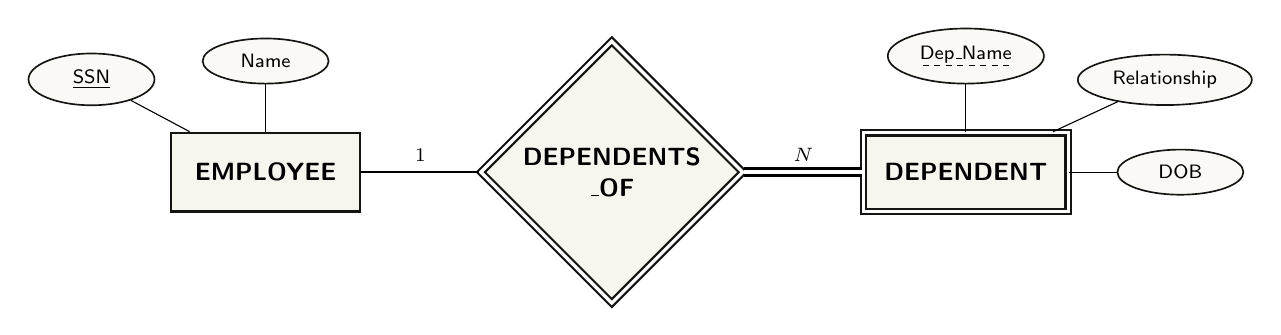
\begin{tikzpicture}[
  entity/.style={rectangle, draw=AnthDark, fill=AnthCardBG, line width=0.8pt, minimum width=2.4cm, minimum height=1.0cm, align=center, font=\small\sffamily\bfseries},
  weakentity/.style={rectangle, draw=AnthDark, double, double distance=1.2pt, fill=AnthCardBG, line width=0.8pt, minimum width=2.6cm, minimum height=1.0cm, align=center, font=\small\sffamily\bfseries},
  rel/.style={diamond, draw=AnthDark, fill=AnthCardBG, line width=0.8pt, minimum width=2.0cm, minimum height=1.0cm, align=center, font=\small\sffamily},
  weakrel/.style={diamond, draw=AnthDark, double, double distance=1.2pt, fill=AnthCardBG, line width=0.8pt, minimum width=2.2cm, minimum height=1.0cm, align=center, font=\small\sffamily\bfseries},
  att/.style={ellipse, draw=AnthDark, fill=AnthLight, line width=0.6pt, minimum width=1.6cm, align=center, font=\scriptsize\sffamily}
]
  \node[entity] (emp) {EMPLOYEE};
  \node[weakrel, right=1.5cm of emp] (has) {DEPENDENTS\\\_OF};
  \node[weakentity, right=1.5cm of has] (dep) {DEPENDENT};

  \draw[line width=0.8pt] (emp) -- node[above, font=\scriptsize\sffamily]{$1$} (has);
  \draw[line width=1.2pt, double, double distance=1.2pt] (has) -- node[above, font=\scriptsize\sffamily]{$N$} (dep);

  %% Attributes
  \node[att, above left=0.6cm of emp] (ssn) {\underline{SSN}};
  \node[att, above=0.6cm of emp] (ename) {Name};
  \draw (emp) -- (ssn);
  \draw (emp) -- (ename);

  \node[att, above=0.6cm of dep] (dname) {\dashuline{Dep\_Name}};
  \node[att, above right=0.6cm of dep] (relat) {Relationship};
  \node[att, right=0.6cm of dep] (dob) {DOB};
  \draw (dep) -- (dname);
  \draw (dep) -- (relat);
  \draw (dep) -- (dob);
\end{tikzpicture}%
}
\end{center}

%% ─────────────────────────────────────────────────────────────────────────────
\subsection{Ternary Relationships (Degree 3)}

A \textbf{Ternary Relationship} represents an atomic association connecting three distinct entity types simultaneously.

\begin{center}
\resizebox{0.65\textwidth}{!}{%
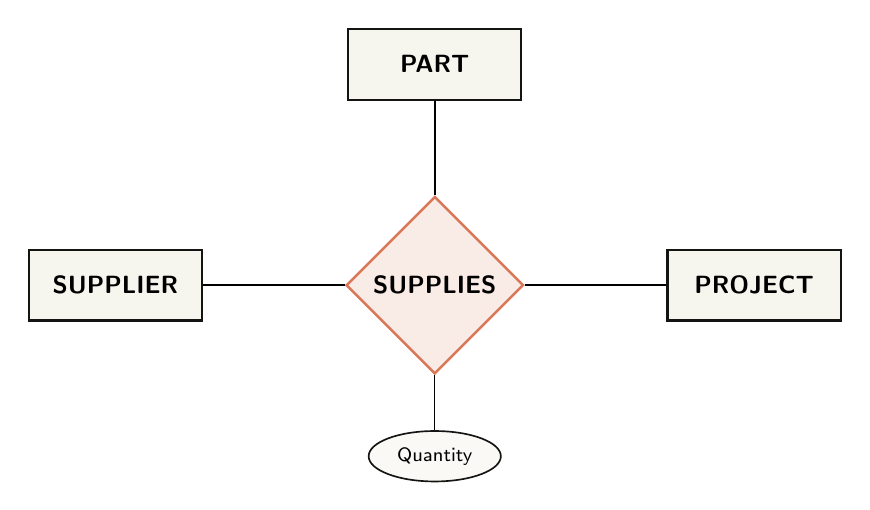
\begin{tikzpicture}[
  entity/.style={rectangle, draw=AnthDark, fill=AnthCardBG, line width=0.8pt, minimum width=2.2cm, minimum height=0.9cm, align=center, font=\small\sffamily\bfseries},
  rel/.style={diamond, draw=AnthOrange, fill=AnthOrange!15, line width=0.9pt, minimum width=2.2cm, minimum height=1.1cm, align=center, font=\small\sffamily\bfseries},
  att/.style={ellipse, draw=AnthDark, fill=AnthLight, line width=0.6pt, align=center, font=\scriptsize\sffamily}
]
  \node[rel] (supply) {SUPPLIES};
  \node[entity, left=1.8cm of supply] (supp) {SUPPLIER};
  \node[entity, right=1.8cm of supply] (proj) {PROJECT};
  \node[entity, above=1.2cm of supply] (part) {PART};

  \draw[line width=0.8pt] (supp) -- (supply);
  \draw[line width=0.8pt] (proj) -- (supply);
  \draw[line width=0.8pt] (part) -- (supply);

  \node[att, below=0.7cm of supply] (qty) {Quantity};
  \draw (supply) -- (qty);
\end{tikzpicture}%
}
\end{center}

\begin{Warn}[Ternary Relationship vs. Three Binary Relationships]
A single ternary relationship \ic{SUPPLIES(Supplier, Part, Project)} cannot generally be decomposed into three binary relationships (\ic{Supplies\_Part}, \ic{Part\_UsedIn\_Project}, \ic{Supplier\_For\_Project}). The ternary relationship captures the exact fact that \emph{Supplier $S_1$ supplied Part $P_1$ specifically for Project $J_1$}, whereas binary combinations only represent pairwise associations without tying all three components together.
\end{Warn}

%% ─────────────────────────────────────────────────────────────────────────────
\clearpage
\subsection{Comprehensive ER Modeling Case Studies}

\begin{Problem}[Case Study 1: Enterprise Company Database]
Design an ER schema for a company with the following requirements:
\begin{itemize}
  \item \ic{DEPARTMENT} has unique name, number (\ic{DNumber}), and multiple locations.
  \item \ic{EMPLOYEE} has \ic{SSN}, name, address, salary, DOB. An employee works in one department and can manage one department. An employee supervises other employees.
  \item \ic{PROJECT} has name, number (\ic{PNumber}), location, controlled by one department. Employees work on multiple projects with recorded hours.
  \item \ic{DEPENDENT} has name, gender, DOB, relationship to employee (weak entity).
\end{itemize}
\end{Problem}

\begin{Solution}
\begin{center}
\resizebox{0.92\textwidth}{!}{%
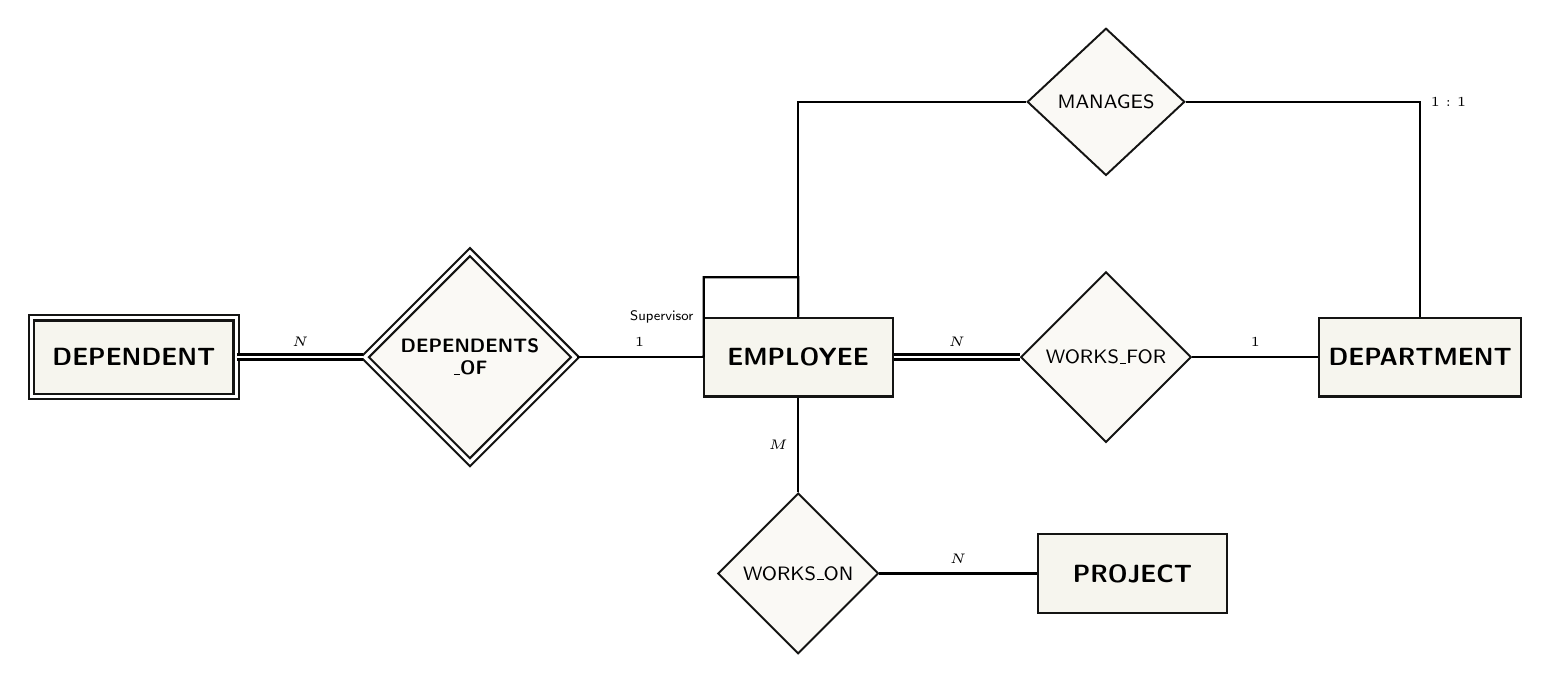
\begin{tikzpicture}[
  entity/.style={rectangle, draw=AnthDark, fill=AnthCardBG, line width=0.8pt, minimum width=2.4cm, minimum height=1.0cm, align=center, font=\small\sffamily\bfseries},
  weakentity/.style={rectangle, draw=AnthDark, double, double distance=1.2pt, fill=AnthCardBG, line width=0.8pt, minimum width=2.6cm, minimum height=1.0cm, align=center, font=\small\sffamily\bfseries},
  rel/.style={diamond, draw=AnthDark, fill=AnthLight, line width=0.7pt, minimum width=2.0cm, minimum height=1.0cm, align=center, font=\scriptsize\sffamily},
  weakrel/.style={diamond, draw=AnthDark, double, double distance=1.2pt, fill=AnthLight, line width=0.8pt, minimum width=2.0cm, minimum height=1.0cm, align=center, font=\scriptsize\sffamily\bfseries}
]
  \node[entity] (emp) {EMPLOYEE};
  \node[rel, right=1.6cm of emp] (works_for) {WORKS\_FOR};
  \node[entity, right=1.6cm of works_for] (dept) {DEPARTMENT};

  \draw[line width=1.2pt, double] (emp) -- node[above, font=\tiny\sffamily]{$N$} (works_for);
  \draw[line width=0.8pt] (works_for) -- node[above, font=\tiny\sffamily]{$1$} (dept);

  \node[rel, above=1.2cm of works_for] (manages) {MANAGES};
  \draw[line width=0.8pt] (emp) |- (manages);
  \draw[line width=0.8pt] (manages) -| node[right, font=\tiny\sffamily]{$1:1$} (dept);

  \node[rel, below=1.2cm of emp] (works_on) {WORKS\_ON};
  \node[entity, right=2.0cm of works_on] (proj) {PROJECT};
  \draw[line width=0.8pt] (emp) -- node[left, font=\tiny\sffamily]{$M$} (works_on);
  \draw[line width=0.8pt] (works_on) -- node[above, font=\tiny\sffamily]{$N$} (proj);

  \node[weakrel, left=1.6cm of emp] (dep_of) {DEPENDENTS\\\_OF};
  \node[weakentity, left=1.6cm of dep_of] (dep) {DEPENDENT};
  \draw[line width=0.8pt] (emp) -- node[above, font=\tiny\sffamily]{$1$} (dep_of);
  \draw[line width=1.2pt, double] (dep_of) -- node[above, font=\tiny\sffamily]{$N$} (dep);

  %% Recursive relationship
  \draw[line width=0.8pt] (emp.north) -- ++(0,0.5) -- ++(-1.2,0) -- node[left, font=\tiny\sffamily]{Supervisor} ++(0,-1.0) -- (emp.west);
\end{tikzpicture}%
}
\end{center}
\end{Solution}

\begin{Problem}[Case Study 2: Television Reality Show Database (KTU Scenario Problem)]
Design an ER schema for TV Reality Shows:
\begin{itemize}
  \item \ic{REALITY\_SHOW}: Name, Genre, Basic\_Info, Participant\_Names ($\ge 2$ participants).
  \item \ic{PRODUCER}: Company\_Name, Company\_Country. A show is produced by exactly 1 producer; 1 producer produces 1 show ($1:1$).
  \item \ic{TELEVISION}: Name, Start\_Year, Head\_Office. Broadcasts multiple shows; each show broadcast by 1 TV ($1:N$).
  \item \ic{USER}: Username, Password, Age. A user rates multiple shows, a show rated by multiple users ($M:N$) with score (0 to 10).
\end{itemize}
\end{Problem}

\begin{Solution}
\begin{enumerate}
  \item \textbf{Entities \& Primary Keys:} \ic{REALITY\_SHOW}(\underline{Show\_ID}, Name, Genre, Basic\_Info), \ic{PRODUCER}(\underline{Company\_Name}, Country), \ic{TELEVISION}(\underline{TV\_Name}, Start\_Year, Head\_Office), \ic{USER}(\underline{Username}, Password, Age).
  \item \textbf{Multivalued Attribute:} \ic{Participants} (double oval connected to \ic{REALITY\_SHOW}).
  \item \textbf{Relationships \& Cardinalities:}
    \begin{itemize}
      \item \ic{PRODUCES}: Binary $1:1$ between \ic{PRODUCER} and \ic{REALITY\_SHOW}.
      \item \ic{BROADCASTS}: Binary $1:N$ between \ic{TELEVISION} and \ic{REALITY\_SHOW}.
      \item \ic{RATES}: Binary $M:N$ between \ic{USER} and \ic{REALITY\_SHOW} with relationship attribute \ic{Rating\_Score}.
    \end{itemize}
\end{enumerate}
\end{Solution}

%% ─────────────────────────────────────────────────────────────────────────────
\clearpage
\section{Physical Data Organization and Indexing Structures}
%% ─────────────────────────────────────────────────────────────────────────────

\syllabusitem{Physical Data Organization - Review of terms: physical and logical records, blocking factor, pinned and unpinned organization. Heap files, Indexing, Singe level indices, numerical examples, Multi-level-indices, numerical examples}

\subsection{Physical Storage Terminology}

Databases are stored permanently on non-volatile secondary storage devices (magnetic hard disks, solid-state drives). Data transfer between disk and main memory (RAM) occurs in fixed-size units called \textbf{Disk Blocks (Pages)}.

\concept{Key Storage Parameters}
\begin{itemize}
  \item \textbf{Logical Record ($R$):} A single data entity tuple consisting of multiple fields (e.g., student record of size $R = 150\,\text{bytes}$).
  \item \textbf{Disk Block Size ($B$):} The fixed unit of physical data transfer (typically $B = 512, 1024, 2048,$ or $4096\,\text{bytes}$).
  \item \textbf{Total Number of Records ($r$):} Number of records in the data file.
\end{itemize}

\concept{Blocking Factor ($bfr$)}
The \textbf{Blocking Factor ($bfr$)} is the number of whole logical records that can be stored in a single disk block:
\begin{equation}
  bfr = \left\lfloor \frac{B}{R} \right\rfloor \quad [\text{records per block}]
\end{equation}
The total number of physical disk blocks ($b$) required to store the data file of $r$ records is:
\begin{equation}
  b = \left\lceil \frac{r}{bfr} \right\rceil \quad [\text{disk blocks}]
\end{equation}
The unused (wasted) space in each disk block is:
\begin{equation}
  \text{Unused Space per Block} = B - (bfr \times R) \quad [\text{bytes}]
\end{equation}

%% ─────────────────────────────────────────────────────────────────────────────
\subsection{Record Placement: Pinned vs. Unpinned (Spanned vs. Unspanned)}

\begin{center}
\small
\begin{tabularx}{\textwidth}{L{3.2cm} L{4.5cm} X}
  \rowcolor{AnthDark}
  \color{white}\textbf{Organization} & \color{white}\textbf{Physical Mechanism} & \color{white}\textbf{Engineering Trade-off} \\
  \rowcolor{AnthCardBG} \textbf{Unspanned (Pinned)} & Each record is contained entirely within a single block. If a record does not fit in remaining block bytes, the space is left unused (padded) and the record starts in the next block. & Simpler record retrieval; no multi-block pointer overhead; wastes space when record size $R$ is large relative to block size $B$. \\
  \textbf{Spanned (Unpinned)} & Records can cross block boundaries. A record starts in one block and continues into the next block using a pointer. & Zero wasted space; mandatory when record size $R > B$; requires two disk block I/Os to read a spanned record. \\
\end{tabularx}
\end{center}

%% ─────────────────────────────────────────────────────────────────────────────
\subsection{Heap Files (Unordered File Organization)}

In a \textbf{Heap File}, records are placed on disk in the order they are inserted. New records are appended to the last block of the file.
\begin{itemize}
  \item \textbf{Insertion Cost:} Fast ($O(1)$ block I/Os, simply write to the last block).
  \item \textbf{Search Cost (Linear Search):}
    \begin{equation}
      \text{Average Block Accesses} = \left\lfloor \frac{b}{2} \right\rfloor, \qquad \text{Worst-Case Block Accesses} = b
    \end{equation}
  \item \textbf{Deletion Cost:} Requires finding the record, setting a deletion flag or moving the last record into the deleted slot.
\end{itemize}

%% ─────────────────────────────────────────────────────────────────────────────
\subsection{Database Indexing Fundamentals}

An \textbf{Index} is an auxiliary access structure built on a search-key field that accelerates data retrieval, reducing search time from linear $O(b)$ to logarithmic $O(\log_2 b)$ or constant $O(1)$.

An index file consists of ordered index entries:
\begin{equation}
  \text{Index Entry} = \langle K_i, P_i \rangle
\end{equation}
where $K_i$ is the search key value and $P_i$ is a block pointer (address of the disk block containing the record).

Let index record size be $R_i = V_K + P_B$ (where $V_K$ is key size and $P_B$ is pointer size). The \textbf{Index Blocking Factor} is:
\begin{equation}
  bfr_i = \left\lfloor \frac{B}{R_i} \right\rfloor \quad [\text{index entries per block}]
\end{equation}

%% ─────────────────────────────────────────────────────────────────────────────
\subsection{Single-Level Ordered Indexes}

\begin{center}
\small
\begin{tabularx}{\textwidth}{L{2.8cm} L{3.5cm} L{3.2cm} X}
  \rowcolor{AnthDark}
  \color{white}\textbf{Index Type} & \color{white}\textbf{Data File Ordering} & \color{white}\textbf{Search Key Field} & \color{white}\textbf{Index Density \& Size} \\
  \rowcolor{AnthCardBG} \textbf{Primary Index} & Ordered by search key & Primary Key (Unique) & \textbf{Sparse Index}: One entry per data block (anchor record). Number of entries $= b$. \\
  \textbf{Clustering Index} & Ordered by search key & Non-Key (Duplicate values) & \textbf{Sparse Index}: One entry per distinct search value. \\
  \rowcolor{AnthCardBG} \textbf{Secondary Index} & Unordered (or ordered on a different field) & Candidate Key / Non-Key & \textbf{Dense Index}: One entry per data record ($r$ entries) for key fields. \\
\end{tabularx}
\end{center}

\begin{Deriv}[Search Cost Comparison: Unordered Heap vs. Primary Index]
Consider a data file with $r = 100,000$ records, record size $R = 200\,\text{bytes}$, block size $B = 2048\,\text{bytes}$.\\
Key size $V_K = 10\,\text{bytes}$, block pointer $P_B = 6\,\text{bytes}$.

1. \textbf{Data File Parameters:}
\begin{equation*}
  bfr = \left\lfloor \frac{2048}{200} \right\rfloor = 10\,\text{records/block}, \qquad b = \left\lceil \frac{100,000}{10} \right\rceil = 10,000\,\text{blocks}
\end{equation*}
2. \textbf{Linear Search on Heap File:}
\begin{equation*}
  \text{Average Cost} = \frac{b}{2} = \frac{10,000}{2} = \mathbf{5,000\,\text{block accesses}}
\end{equation*}
3. \textbf{Primary Index Parameters (Sparse):}
\begin{equation*}
  R_i = 10 + 6 = 16\,\text{bytes}, \qquad bfr_i = \left\lfloor \frac{2048}{16} \right\rfloor = 128\,\text{entries/block}
\end{equation*}
Number of primary index entries $= b = 10,000$. Total index blocks ($b_i$):
\begin{equation*}
  b_i = \left\lceil \frac{10,000}{128} \right\rceil = 79\,\text{index blocks}
\end{equation*}
4. \textbf{Binary Search using Primary Index:}
\begin{equation*}
  \text{Cost} = \lceil \log_2(b_i) \rceil + 1 = \lceil \log_2(79) \rceil + 1 = 7 + 1 = \mathbf{8\,\text{block accesses}}
\end{equation*}
\emph{Result:} Indexing reduces disk I/O from \textbf{5,000 block accesses down to just 8 block accesses (a 625× speedup!)}.
\end{Deriv}

%% ─────────────────────────────────────────────────────────────────────────────
\subsection{Multi-Level Indexes and B/B+ Trees}

When the primary index file itself becomes too large to fit in main memory, a \textbf{Second-Level Index} is created on top of the primary index, treating the primary index as a data file. This process is repeated hierarchically until the top-level index fits in a single block (the root block).

\begin{Def}[Multi-Level Index Fan-Out and Tree Height]
The \textbf{Fan-Out ($fo$)} of an index block is the number of pointers it can store:
\begin{equation}
  fo = bfr_i = \left\lfloor \frac{B}{V_K + P_B} \right\rfloor
\end{equation}
For a base index of $b_1$ blocks, the number of index levels ($x$) is:
\begin{equation}
  x = \left\lceil \log_{fo}(b_1) \right\rceil + 1
\end{equation}
Total Block Accesses to retrieve a record $= x + 1$ (where $+1$ is for the final data block).
\end{Def}

%% ─────────────────────────────────────────────────────────────────────────────
\clearpage
\section{Comprehensive Numerical Problem Suite}
%% ─────────────────────────────────────────────────────────────────────────────

\begin{Problem}[Problem 1: Blocking Factor and File Storage Size]
A customer data file contains $r = 50,000$ fixed-length records. Each record has size $R = 250\,\text{bytes}$. The disk block size is $B = 4096\,\text{bytes}$. Calculate: (a) Blocking factor ($bfr$), (b) Total number of disk blocks ($b$) using unspanned organization, (c) Total wasted storage space across the file, and (d) Average block accesses to search a record in heap organization.
\end{Problem}

\begin{Solution}
\begin{enumerate}
  \item Blocking Factor:
    \begin{equation*}
      bfr = \left\lfloor \frac{B}{R} \right\rfloor = \left\lfloor \frac{4096}{250} \right\rfloor = \lfloor 16.384 \rfloor = \mathbf{16\,\text{records/block}}
    \end{equation*}
  \item Total Data Blocks:
    \begin{equation*}
      b = \left\lceil \frac{r}{bfr} \right\rceil = \left\lceil \frac{50,000}{16} \right\rceil = \lceil 3125 \rceil = \mathbf{3,125\,\text{blocks}}
    \end{equation*}
  \item Wasted Space:
    \begin{align*}
      \text{Unused bytes per block} &= 4096 - (16 \times 250) = 4096 - 4000 = 96\,\text{bytes} \\
      \text{Total Wasted Space} &= 3,125 \times 96\,\text{bytes} = \mathbf{300,000\,\text{bytes}} \approx \mathbf{300\,\text{kB}}
    \end{align*}
  \item Average Linear Search Accesses (Heap):
    \begin{equation*}
      \text{Cost} = \left\lfloor \frac{b}{2} \right\rfloor = \left\lfloor \frac{3125}{2} \right\rfloor = \mathbf{1,562\,\text{block accesses}}
    \end{equation*}
\end{enumerate}
\end{Solution}

\begin{Problem}[Problem 2: Primary Index Storage and Search Performance]
For the file in Problem 1, suppose the records are ordered on a primary key field of size $V_K = 14\,\text{bytes}$. Block pointers take $P_B = 6\,\text{bytes}$. Construct a primary index and calculate: (a) Number of index entries, (b) Index blocking factor, (c) Number of index blocks ($b_i$), and (d) Total block accesses to find a record using binary search on the index.
\end{Problem}

\begin{Solution}
\begin{enumerate}
  \item Primary Index is \textbf{sparse} (one entry per data block).
    \begin{equation*}
      \text{Number of Index Entries} = b = \mathbf{3,125\,\text{entries}}
    \end{equation*}
  \item Index record size: $R_i = V_K + P_B = 14 + 6 = 20\,\text{bytes}$.
  \item Index Blocking Factor:
    \begin{equation*}
      bfr_i = \left\lfloor \frac{B}{R_i} \right\rfloor = \left\lfloor \frac{4096}{20} \right\rfloor = \lfloor 204.8 \rfloor = \mathbf{204\,\text{entries/block}}
    \end{equation*}
  \item Number of Index Blocks:
    \begin{equation*}
      b_i = \left\lceil \frac{3,125}{204} \right\rceil = \lceil 15.318 \rceil = \mathbf{16\,\text{index blocks}}
    \end{equation*}
  \item Binary Search Block Accesses:
    \begin{equation*}
      \text{Cost} = \lceil \log_2(b_i) \rceil + 1 = \lceil \log_2(16) \rceil + 1 = 4 + 1 = \mathbf{5\,\text{block accesses}}
    \end{equation*}
\end{enumerate}
\end{Solution}

\begin{Problem}[Problem 3: Secondary Index on a Non-Ordering Key Field]
Suppose an unordered employee file of $r = 100,000$ records has record size $R = 100\,\text{bytes}$ and block size $B = 2048\,\text{bytes}$. A secondary index is built on a non-ordering unique SSN field of size $V_K = 12\,\text{bytes}$ and record pointer $P_R = 8\,\text{bytes}$. Calculate: (a) Total data blocks, (b) Total secondary index blocks, and (c) Search cost comparison between heap linear search and secondary index.
\end{Problem}

\begin{Solution}
\begin{enumerate}
  \item Data File Parameters:
    \begin{equation*}
      bfr = \left\lfloor \frac{2048}{100} \right\rfloor = 20\,\text{records/block}, \qquad b = \left\lceil \frac{100,000}{20} \right\rceil = \mathbf{5,000\,\text{data blocks}}
    \end{equation*}
  \item Secondary Index is \textbf{dense} (one entry per data record):
    \begin{equation*}
      \text{Number of Index Entries} = r = 100,000
    \end{equation*}
    Index entry size: $R_i = V_K + P_R = 12 + 8 = 20\,\text{bytes}$.
    \begin{equation*}
      bfr_i = \left\lfloor \frac{2048}{20} \right\rfloor = 102\,\text{entries/block}
    \end{equation*}
    Total secondary index blocks:
    \begin{equation*}
      b_i = \left\lceil \frac{100,000}{102} \right\rceil = \lceil 980.39 \rceil = \mathbf{981\,\text{index blocks}}
    \end{equation*}
  \item Search Cost Comparison:
    \begin{itemize}
      \item \textbf{Unordered Heap Search:} Average $\lfloor b/2 \rfloor = \mathbf{2,500\,\text{block accesses}}$.
      \item \textbf{Secondary Index Search:} $\lceil \log_2(b_i) \rceil + 1 = \lceil \log_2(981) \rceil + 1 = 10 + 1 = \mathbf{11\,\text{block accesses}}$.
    \end{itemize}
\end{enumerate}
\end{Solution}

\begin{Problem}[Problem 4: Multi-Level Index Access Cost]
A large data file has $b = 1,000,000$ data blocks. A multi-level index is constructed with block size $B = 4096\,\text{bytes}$, search key size $V_K = 26\,\text{bytes}$, and block pointer $P_B = 6\,\text{bytes}$. Determine: (a) Fan-out of the index, (b) Number of index blocks at each level, (c) Number of levels in the index tree, and (d) Total disk block accesses to retrieve any record.
\end{Problem}

\begin{Solution}
\begin{enumerate}
  \item Fan-Out ($fo$):
    \begin{equation*}
      R_i = 26 + 6 = 32\,\text{bytes} \implies fo = bfr_i = \left\lfloor \frac{4096}{32} \right\rfloor = \mathbf{128\,\text{entries/block}}
    \end{equation*}
  \item Multi-Level Index Hierarchy:
    \begin{itemize}
      \item \textbf{Level 1 Index Blocks ($b_1$):} $\lceil \frac{b}{fo} \rceil = \lceil \frac{1,000,000}{128} \rceil = \mathbf{7,813\,\text{blocks}}$.
      \item \textbf{Level 2 Index Blocks ($b_2$):} $\lceil \frac{b_1}{fo} \rceil = \lceil \frac{7,813}{128} \rceil = \mathbf{62\,\text{blocks}}$.
      \item \textbf{Level 3 Index Blocks ($b_3$):} $\lceil \frac{b_2}{fo} \rceil = \lceil \frac{62}{128} \rceil = \mathbf{1\,\text{block}}$ (Root level reached!).
    \end{itemize}
  \item Total Index Levels: $x = \mathbf{3\,\text{levels}}$.
  \item Total Disk Accesses to retrieve record $= x + 1 = 3 + 1 = \mathbf{4\,\text{block accesses}}$ (Level 3 root $\to$ Level 2 $\to$ Level 1 $\to$ Data Block).
\end{enumerate}
\end{Solution}

%% ─────────────────────────────────────────────────────────────────────────────
\clearpage
\section{Quick Revision Sheet \& Model Examination Questions}
%% ─────────────────────────────────────────────────────────────────────────────

\subsection{Master Summary Table of ER Notations and Physical Storage Formulas}

\begin{center}
\small
\begin{tabularx}{\textwidth}{L{3.2cm} L{4.5cm} X}
  \rowcolor{AnthDark}
  \color{white}\textbf{Concept} & \color{white}\textbf{Notation / Formula} & \color{white}\textbf{Meaning \& Description} \\
  \rowcolor{AnthCardBG} \textbf{Strong Entity} & Rectangle & Entity with a primary key attribute \\
  \textbf{Weak Entity} & Double Rectangle & Dependent entity without primary key of its own \\
  \rowcolor{AnthCardBG} \textbf{Partial Key} & Dashed Underline (\dashuline{Attr}) & Discriminator within identifying entity set \\
  \textbf{Relationship} & Diamond & Association among entities \\
  \rowcolor{AnthCardBG} \textbf{Identifying Rel} & Double Diamond & Relates weak entity to owner entity \\
  \textbf{Multivalued Attr} & Double Oval & Attribute with set of multiple values \\
  \rowcolor{AnthCardBG} \textbf{Derived Attribute} & Dashed Oval & Dynamically computed attribute \\
  \textbf{Total Participation} & Double Line & Existence dependency ($min \ge 1$) \\
  \rowcolor{AnthCardBG} \textbf{Blocking Factor} & $bfr = \lfloor B / R \rfloor$ & Records per physical disk block \\
  \textbf{Primary Index} & $b_i = \lceil b / bfr_i \rceil$ & Sparse index on ordered primary key \\
  \rowcolor{AnthCardBG} \textbf{Secondary Index} & $b_i = \lceil r / bfr_i \rceil$ & Dense index on candidate key \\
  \textbf{Multi-Level Cost} & Cost $= x + 1$ block I/Os & $x = \lceil \log_{fo}(b_1) \rceil + 1$ levels in index tree \\
\end{tabularx}
\end{center}

\subsection{Model Examination Questions (KTU S5 Pattern)}

\begin{Warn}[University Examination Pattern (PBEOT504 Scheme)]
The End Semester Examination consists of \textbf{Part A} (8 compulsory questions of 2 marks each, 2 from each module) and \textbf{Part B} (Module choice questions carrying 6 marks each).
\end{Warn}

\concept{Part A: Short Answer Questions (2 Marks Each)}
\begin{enumerate}
  \item \textbf{Q1:} State two major limitations of traditional file processing systems that are overcome by a DBMS.
  \item \textbf{Q2:} Differentiate between \emph{Logical Data Independence} and \emph{Physical Data Independence}. Which one is more difficult to achieve and why?
  \item \textbf{Q3:} Define a \emph{Weak Entity Type}. How is it represented in an ER diagram?
  \item \textbf{Q4:} What is meant by \emph{Blocking Factor} ($bfr$)? How does it affect total disk blocks required for a data file?
  \item \textbf{Q5:} Differentiate between a \emph{Primary Index} and a \emph{Secondary Index} in terms of file ordering and index density.
  \item \textbf{Q6:} Explain the $(min, max)$ notation used to represent structural constraints in ER diagrams.
\end{enumerate}

\concept{Part B: Long Answer / Analytical Questions (6 Marks Each)}
\begin{enumerate}
  \item \textbf{Q7 (a):} Explain the ANSI/SPARC Three-Schema Architecture with a neat diagram. Describe the role of mappings between adjacent schema levels. \hfill (4 Marks) \\
  \textbf{Q7 (b):} Classify structured, semi-structured, and unstructured data with suitable examples. \hfill (2 Marks)
  
  \item \textbf{Q8 (a):} A company database records information about projects, employees, and departments. An employee has an ID, name, and address. A department has a department number and name. A project has a project number and location. An employee works in one department, manages at most one department, and works on multiple projects with recorded hours. Draw the complete ER diagram showing keys, cardinality ratios, and participation constraints. \hfill (6 Marks)

  \item \textbf{Q9 (a):} A data file contains $40,000$ records of size $200\,\text{bytes}$ each. The block size is $2048\,\text{bytes}$. A primary index is built on a key field of $14\,\text{bytes}$ with block pointer size of $6\,\text{bytes}$. Calculate: (i) Blocking factor of data file and index file, (ii) Total data blocks and index blocks, and (iii) Number of block accesses to search a record using binary search on the index compared to linear search on the heap file. \hfill (6 Marks)
\end{enumerate}

\vfill
\begin{center}
\small\sffamily\color{AnthMidGray}
--- End of Module 1 Study Notes ---
\end{center}

\end{document}
